\subsection{Functional failure study}
\label{sec:failure-case-study}

% How is the failure produced
The failure is observed on the V\textsubscript{2p5} output pin (Fig. \ref{fig:meas-reset-v2p5}).
A negative \gls{tlp} pulse is injected on top of the \gls{dc} supply, connected to the input pin V\textsubscript{batt}.
The width of the discharge is the usual 100 ns, with a risetime of 1 ns.
Failures start to appear with pulse amplitudes larger than -80 V.
To perform the injection, the battery is replaced by a \gls{dc} source and a \gls{tlp} generator.
Both devices are isolated from one another using a \gls{bias-tee}, as defined in the DPI standard \cite{iec62132-4}.
This setup is simply a capacitor-inductor network as shown in Fig. \ref{fig:injection-setup-dpi}.

\begin{figure}[!h]
  \centering
  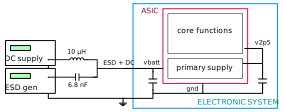
\includegraphics{src/3/figures/architecture_system_test.pdf}
  \caption{Injection setup to superimpose a stress on a DC voltage}
  \label{fig:injection-setup-dpi}
\end{figure}

% What is the root cause -> reset of regulator, soft-start
The failure signature recorded on V\textsubscript{2p5} is given in Fig. \ref{fig:meas-reset-v2p5}.
The area of the curve in red corresponds to the entire restart.
The nominal value for V\textsubscript{2p5} is 2.5 V.
The \gls{tlp} pulse is visible at 53 \textmu{}s.
After a small delay of about 2 \textmu{}s, the regulation function slowly shuts down.
The output voltage falls for nearly 30 \textmu{}s until reaching a voltage of 1.5 V.
At this point, the supply cannot reliably power digital gates for instance, and is completely at fault.
Afterwards, a new soft-start sequence begins.
A soft-start normally happens only during system power-up, when the main external supply is switched on.
During a soft-start, the supply voltage slowly rises from 0 V to its nominal value.
It avoids overshoots that could damage sensitive blocks, and is a slow procedure that takes tens of microseconds to complete.
The shut-down followed by the soft-start last in total about 50 \textmu{}s
It corresponds to the time it takes for the signal V\textsubscript{2p5} to recover.
In comparison, the input disturbance on V\textsubscript{batt} lasts only 100 ns.

\begin{figure}[!h]
  \centering
  \includegraphics[width=0.9\textwidth]{src/3/figures/v2p5_measure.png}
  \caption{Measurement of V\textsubscript{2p5} after a -100V 100ns negative stress}
  \label{fig:meas-reset-v2p5}
\end{figure}

% Discuss lack of impact of positive stress
Testing was also conducted using positive stresses, however no failure could be triggered up the maximum discharge level.
The integrated circuit seems much more sensitive to negative discharges.
After this preliminary testing on a real chip, the analysis is conducted with simulation tools to understand how the failure appears internally.

% Compare sim and meas for Vbatt
A transient simulation of the integrated regulation function is ran.
It uses the transistor-level schematic of the function, and its surrounding environment composed of decoupling capacitors, printed cricuit board, \gls{dc} sources and test generator.
The simulation of V\textsubscript{batt} is compared to a measurement in Fig. \ref{fig:wvf-vbatt}.
The simulation setup reproduces the measurement setup, using the modelling approach presented in previous chapter.
During the discharge, V\textsubscript{batt} has a larger amplitude in simulation, and reaches a more negative voltage.
The positive overshoot after the pulse is correctly reproduced, although it dampens slower in the simulation.
It looks like the measurement has less bandwidth than the simulation.
The accuracy is not great, but it is sufficient to reproduce the failure on the output.
Also, the timescale is much sorter than in Fig. X and the analysis focuses here on events longer than a few microseconds.

\begin{figure}[!h]
  \centering
  \includegraphics[width=0.95\textwidth]{src/3/figures/vbatt.png}
  \caption{Measurement and simulation for V\textsubscript{batt} (short timescale)}
  \label{fig:wvf-vbatt}
\end{figure}

% Compare sim and meas for V2p5
Fig. \ref{fig:wvf-v2p5} provides the same comparison for V\textsubscript{2p5}.
The reset is clearly visible on both simulation and measurement.
The restart happens almost at the same time in both waveforms, at about 32\textmu{}s after the stress was injected.
Right after the \gls{esd} injection, the disturbance amplitude is a bit larger in simulation.
But overall, the accuracy is satisfying.
Both comparisons tend to indicate that simulations can be trusted to reproduce the failure in this study case.

\begin{figure}[!h]
  \centering
  \includegraphics[width=0.9\textwidth]{src/3/figures/v2p5.png}
  \caption{Measurement and simulation of the functional failure on V\textsubscript{2p5}}
  \label{fig:wvf-v2p5}
\end{figure}

% Now use the simulation for analysis
So far, the waveforms of V\textsubscript{batt} (external input) and V\textsubscript{2p5} (external output) were shown.
Simulations are now employed to observe the intermediate nets inside the integrated circuit.
The waveform for the internal output V\textsubscript{clamp9} of the pre-regulator is given in Fig. \ref{fig:wvf-vclamp9}.
The timescale is shorter than the previous curves.
At 54 \textmugreek{}s,  V\textsubscript{clamp9} is disturbed by the negative stress, in two phases.
The first phase is 100 ns wide, and corresponds to the direct exposure to the stress.
During this phase, V\textsubscript{clamp9} reaches as low as 0V for a brief amount of time.
Afterwards, there is a second phase, that lasts approximately 650 ns.
This second undervoltage will not be detailed but can be explained by the design and architecture of the block.
Overall, V\textsubscript{clamp9} is disturbed for 750 ns.

\begin{figure}[!h]
  \centering
  \includegraphics[width=0.95\textwidth]{src/3/figures/vclamp9.png}
  \caption{Simulated waveform of the V\textsubscript{clamp9} internal net (short timescale)}
  \label{fig:wvf-vclamp9}
\end{figure}

% Next net, bandgap input
V\textsubscript{clamp9} is used as a power supply for the bandgap reference.
The bandgap is expected to be disturbed because of the variation on V\textsubscript{clamp9}.
The observation of the 1.0V bandgap reference V\textsubscript{ref1p0} confirms it (Fig. \ref{fig:wvf-v1p0}).
The reference drops down to 0.25V, and is disturbed for about 3 \textmugreek{}s.

\begin{figure}[!h]
  \centering
  \includegraphics[width=0.9\textwidth]{src/3/figures/v1p0.png}
  \caption{Simulated waveform of the V\textsubscript{ref1p0} internal net}
  \label{fig:wvf-v1p0}
\end{figure}

% Final net
Finally, V\textsubscript{ref1p0} is used by the regulator to generate the 2.5 V external supply output V\textsubscript{2p5}.
Previously,  Fig. \ref{fig:wvf-v2p5} showed that V\textsubscript{2p5} drops below 1.5V, and is disturbed for more than 30 \textmugreek{}s.

% Preliminary conclusion with scale factor
There is a clear trend regarding the duration of the failure.
In the first block (pre-regulator), the disturbance width increased from 100 ns to 750 ns.
In the second block (bandgap), it increased from 750 ns to 3 \textmugreek{}s.
In the third block (regulator), it reached 30 \textmugreek{}s.
After each block, there is an aggravation or an amplification of the failure.
Ultimately, the final regulation function that takes a lot of time to recover is hit, causing a full system restart.

% Transition
The next part of this research work is focused on developping measurement methods to acquire data at the silicon level, to confirm the simulations.
A testchip is designed to test new measurement and observation methods in section \ref{sec:test-vehicle-desc}.
Modeling methods are explored in section \ref{sec:bottom-up-modeling} as a way to understand and predict these functional issues.
